\documentclass[ngerman,compress,aspectratio=169]{beamer}

\usepackage{hyperref}
\usepackage{graphicx}
\graphicspath{{img/}}

\mode<presentation>
{
  \useoutertheme[footline=titleinstituteauthor]{c4}
  \useinnertheme{circles}
  \usecolortheme{c4}
  %\setbeamercovered{transparent}
  \setbeamercovered{highly dynamic}
}

\usepackage{babel}
\usepackage[utf8]{inputenc}
\usepackage{fontspec}
\setsansfont{DejaVu Sans}

\usepackage{bytefield}

\usepackage[binary-units]{siunitx}
\DeclareSIUnit \Byte {Byte}

\usepackage{hyperref}

\title[Projekt Netzwerk-Monitoring - u23 2014]
{\textbf{Projekt Netzwerk-Monitoring: \\ BATMAN und collectd} \\u23 2014}

%\title[collectd, RRD und ein BATMAN-Plugin f\"ur collectd - u23 2014]
%{\textbf{collectd, RRD und \\ ein BATMAN-Plugin f\"ur collectd} \\u23 2014}

\author[mraerino, esssing]
{mraerino, esssing}

\institute[Chaos Computer Club Cologne]
{
Chaos Computer Club Cologne e.V.\\
\url{https://koeln.ccc.de}
}

\date{2014-11-27}

\pgfdeclareimage[height=1cm]{barcode}{./c4-logo}
\logo{\pgfuseimage{barcode}}

\AtBeginSection[]
{
\begin{frame}<beamer>
	\tableofcontents[currentsection,currentsubsection]
\end{frame}
}

\newcommand{\code}[1]{\texttt{#1}}


\begin{document}

\begin{frame}
	\titlepage
\end{frame}

\begin{frame}
	\tableofcontents
\end{frame}

\section{collectd}

\begin{frame}{Was ist collectd?}
	\begin{itemize}
		\pause
		\item ein Deamon
		\pause
		\item sammelt Daten \"uber das System
		\pause
		\item und speichert diese
	\end{itemize}
	%\begin{center}
	%	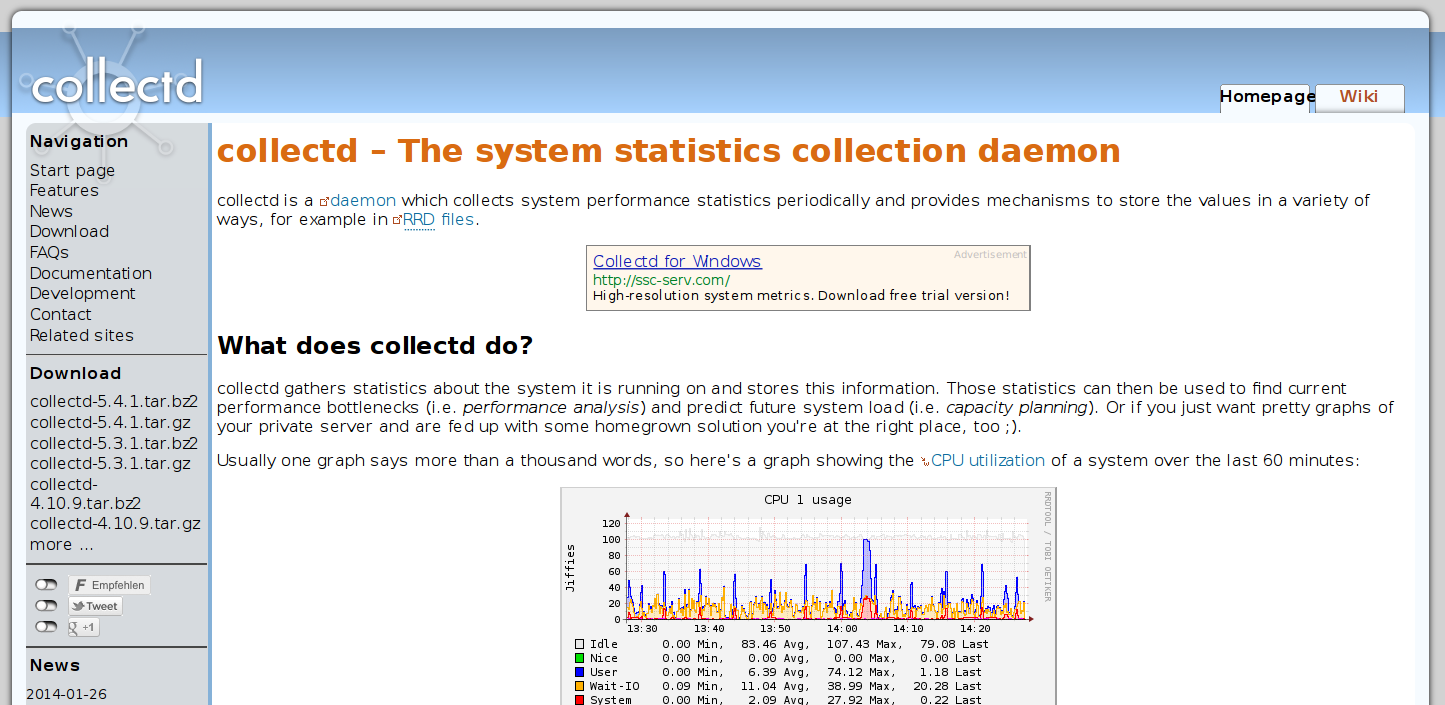
\includegraphics[scale=0.28]{collectd}
	%\end{center}
\end{frame}

\begin{frame}{Modularit\"at}
	\begin{center}
		fast alles sind Plugins!
	\end{center}
	\begin{center}
		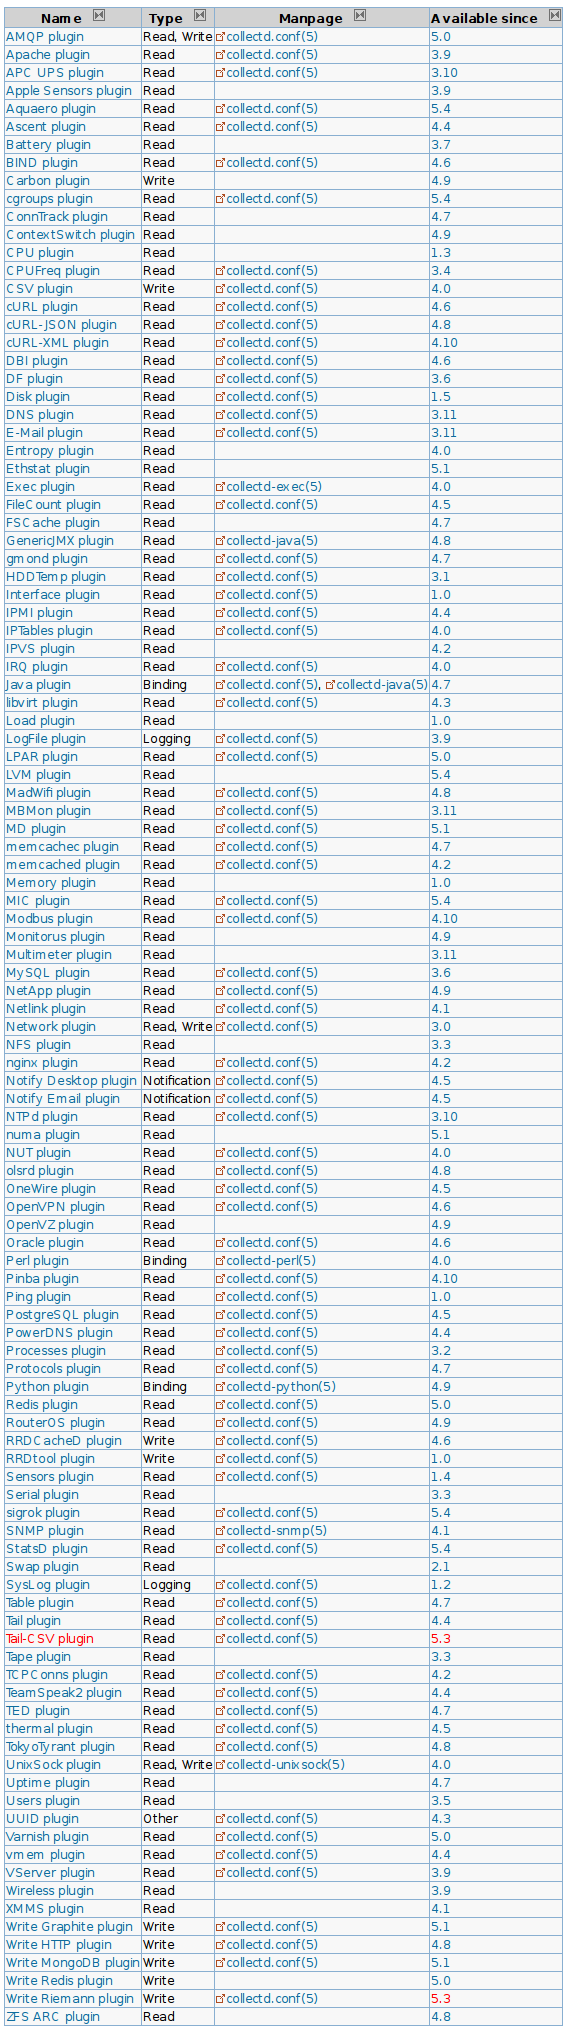
\includegraphics[scale=0.40]{plugins}
	\end{center}
\end{frame}

\begin{frame}{Plugin-Architektur}
	Plugins m\"ussen (bzw.\ k\"onnen) Callbacks implementieren:
	\begin{itemize}
		\pause
		\item config
		\pause
		\item init
		\pause
		\item log
		\pause
		\item \textbf{read}
		\pause
		\item write
		\pause
		\item shutdown
		\pause
		\item $\ldots$
	\end{itemize}
\end{frame}

\section{RRD}

\begin{frame}{round-robin database}
	\begin{itemize}
		\pause
		\item Datenpunkte mit konstanten Zeitabst\"anden
		\pause
		\item feste Datenmenge / Dateigr\"o\ss e
		\pause
		\item \glqq wrap around\grqq, wenn die Datei \glqq voll\grqq\ ist
		\pause
	\end{itemize}
\end{frame}

\begin{frame}{rrdtool}
	\begin{itemize}
		\pause
		\item neue RRD-Dateien erzeugen
		\pause
		\item vorhandene RRD-Dateien mit neuen Werten aktualisieren
		\pause
		\item die Daten aus einer Datei dumpen
		\pause
		\item $\ldots$
		\pause
		\item \textbf{Graphen plotten}
	\end{itemize}
\end{frame}

\begin{frame}{Verwendung in FF-KBU / cserv}
	\begin{center}
		\url{https://kbu.freifunk.net/cserv}
	\end{center}
	%\begin{center}
	%	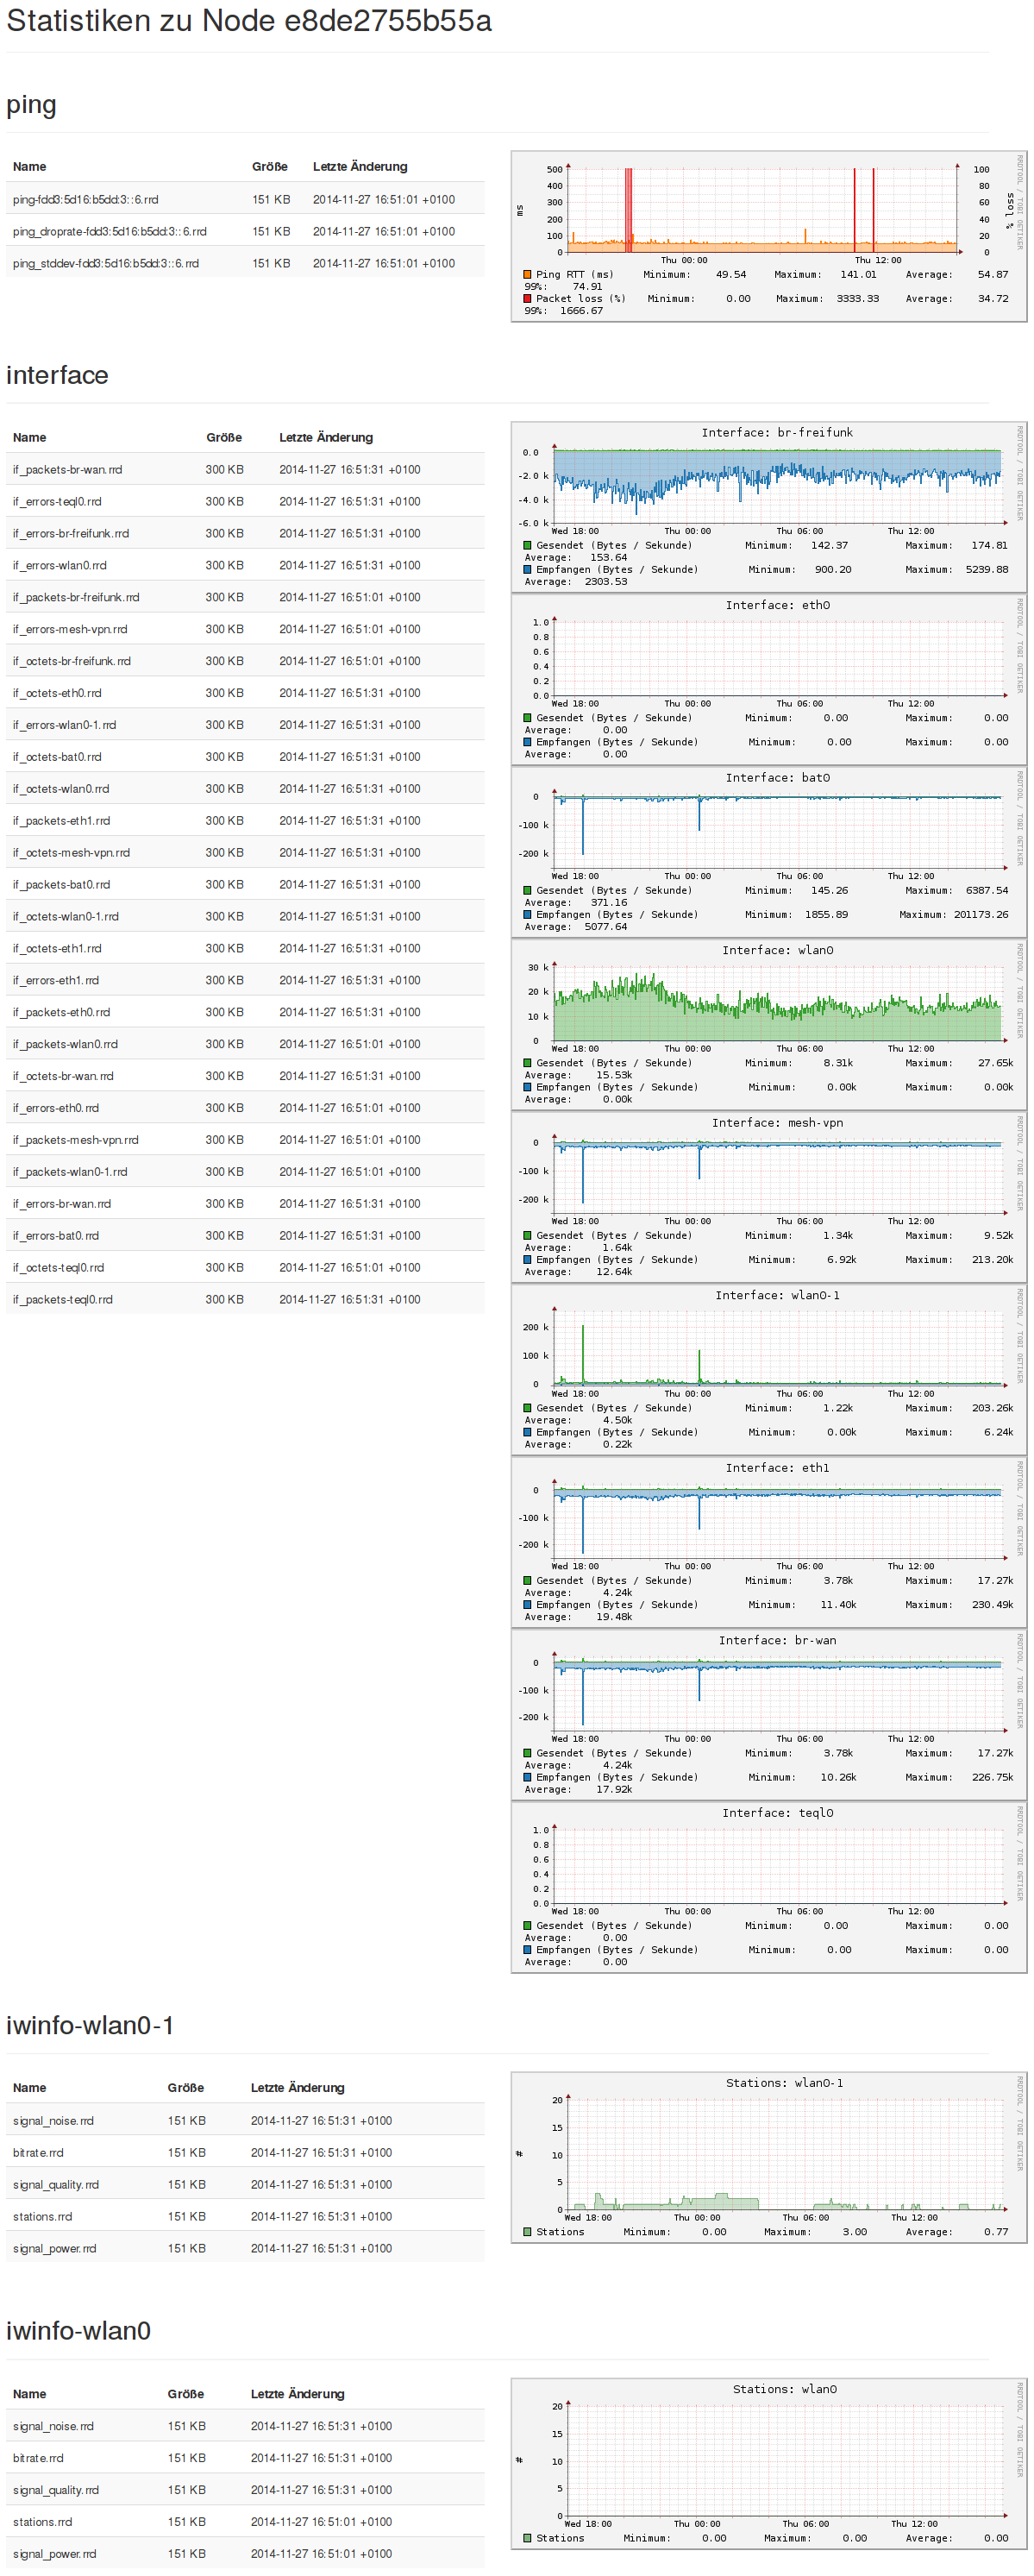
\includegraphics[scale=0.25]{cserv}
	%\end{center}
\end{frame}

\section{das Plugin}

\end{document}

